\documentclass{article}
\usepackage[T1,T2A]{fontenc}
\usepackage[utf8]{inputenc}
\usepackage[english,ukrainian]{babel}
\usepackage[]{amsthm} %lets us use \begin{proof}
\usepackage[]{amssymb} %gives us the character \varnothing
\usepackage{graphicx}

\begin{document}

\title{Семінар 10. Графи. Початок :)}
\date{2 червня 2023}

\maketitle

\subsection*{Графи в реальному житті}
\begin{itemize}
    \item Соцмережі, шість рукостискань, числе Ердеша, гра в Вікіпедію
    \item Складання розкладу
    \item Графові бази даних
    \item Граф знань
\end{itemize}

\subsection*{Трохи нових означень}
\begin{itemize}
    \item сусідні вершини, петля, степінь вершини, ізольована вершина
    \item двудольний граф, парування
\end{itemize}

\subsection*{Задача}
\begin{itemize}
    \item Намалюйте граф у якого 4 вершини зі степенями 1,2,3,4
    \item Чи можна цей граф намалювати без петель?
    \item Намалюйте граф без петель у якого 5 вершин зі степенням 4,1,1,1,1
    \item Намалюйте граф без петель у якого 6 вершин зі степенням 5,5,5,5,1
\end{itemize}

\begin{figure}[ht!]
\centering
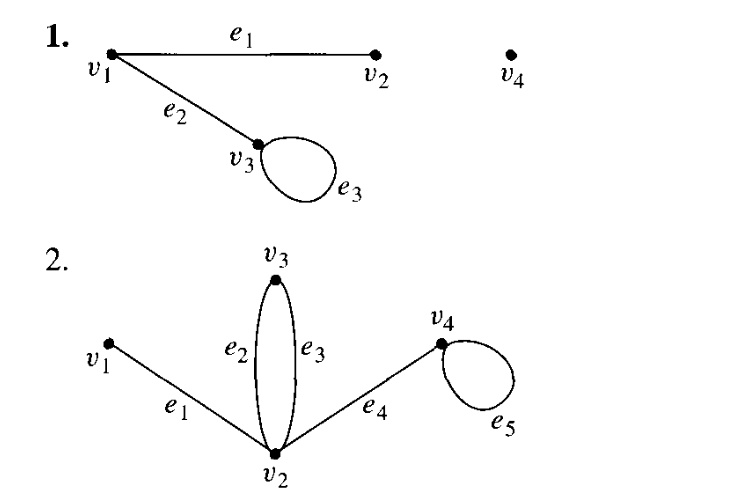
\includegraphics[width=90mm]{1}
\caption{Запишіть граф за допомогую матриці}
\end{figure}

\begin{figure}[ht!]
\centering
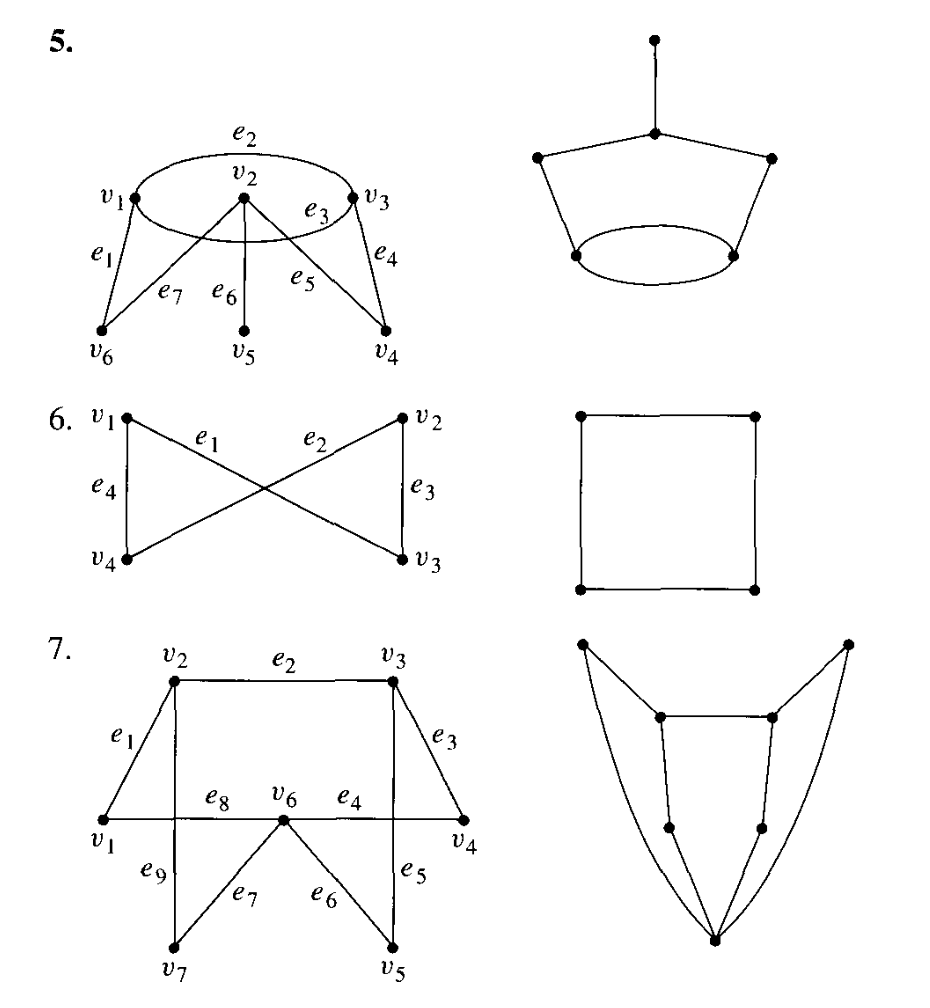
\includegraphics[width=90mm]{2}
\caption{Покажіть що графи однакові позначивши ребра і вершини на графах справа}
\end{figure}

\begin{figure}[ht!]
\centering
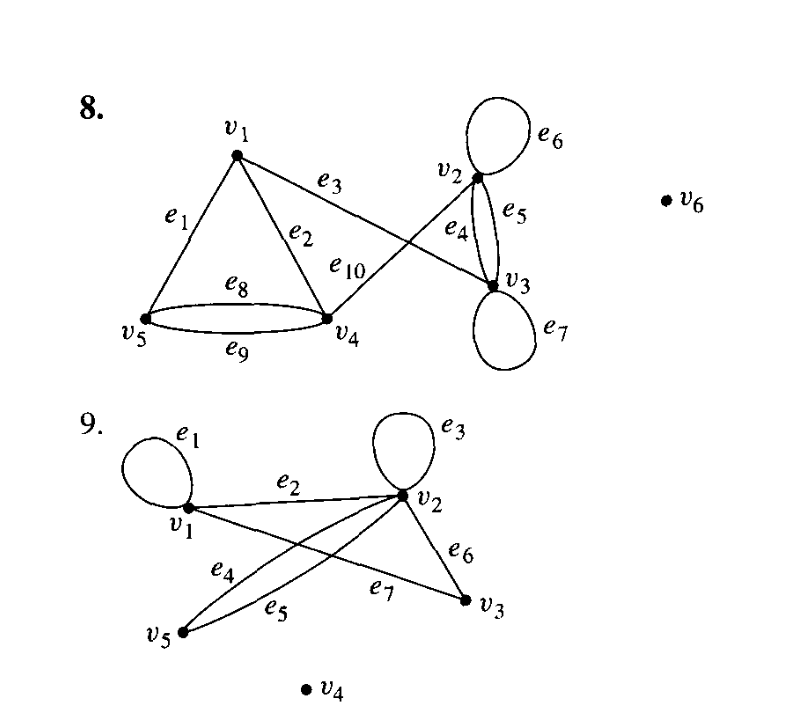
\includegraphics[width=90mm]{4}
\caption{Знайдіть: ребра, що виходять з $v_1$, сусідів $v_3$, петлі, ізольовані вершини, степінь $v_3$}
\end{figure}

\begin{figure}[ht!]
\centering
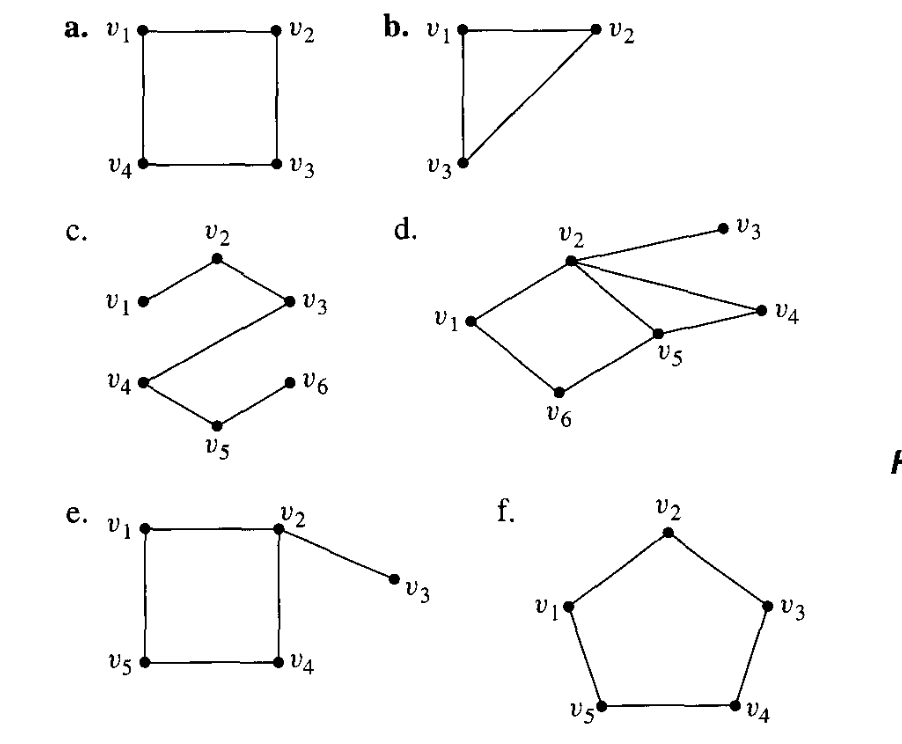
\includegraphics[width=90mm]{5}
\caption{Які з цих графів двудольні? Для двудольних вкажіть долі}
\end{figure}

\end{document}